\chapter{Evaluation}
This chapter will discuss the experiments performed, as well as the ideas and intuitions behind them. The adversarial algorithm will be refined throughout the different subsections and the results of the refinement will be discussed at the end of each subsection.

\section{Evaluation protocol}
This subsection described the evaluation protocol that will be followed for all experiments performed. Experiments will be performed with the MNIST \cite{mnist} and CIFAR \cite{cifar} datasets. Some examples of these datasets are visualised in Figures \ref{fig:mnist} and \ref{fig:cifar} respectively. A black box model is trained using the training data of the respective dataset. The architectures of the models are identical to the ones used in \cite{cw_attack, defensive_distillation}. A summary of the two architectures can be found in Table \ref{tbl:architectures}. The training parameters are also identical to the ones used in \cite{cw_attack, defensive_distillation}. These models remain unchanged for all experiments.\\

The trained models are then used to classify all instances in the test set of their respective dataset. The incorrectly classified examples are filtered out of this set as they are essentially already adversarial. The remaining examples can be used for experiments. A list of experiments is generated based on the remaining examples. An experiment consists of an original image, a target label and starting position(s). All future refinements will therefore perform the same set of experiments in order to make the comparison more fair. All random effects present in the algorithm are seeded for the same purpose.\\

\begin{figure}
\centering
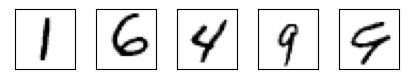
\includegraphics[width=\textwidth]{Images/mnist.png}
\caption[Some examples of the MNIST dataset]{Some examples of the MNIST dataset.}
\label{fig:mnist}
\end{figure}

\begin{figure}
\centering
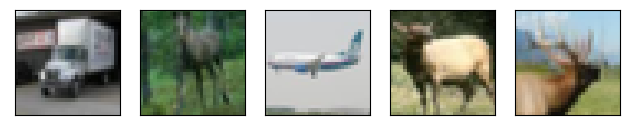
\includegraphics[width=\textwidth]{Images/cifar.png}
\caption[Some examples of the CIFAR-10 dataset]{Some examples of the CIFAR-10 dataset.}
\label{fig:cifar}
\end{figure}

\begin{table}
	\centering
	\caption[Model architectures for the MNIST and CIFAR model]{Model architectures for the MNIST and CIFAR models. The architectures are identical to \cite{cw_attack, defensive_distillation}.}
    \begin{tabular}{lll}\toprule
        Layer type     & MNIST Model &CIFAR Model\\ \midrule
		Convolution + \gls{relu}	&$3 \times 3 \times 32$ &$3\times3\times64$\\
		Convolution + \gls{relu}	&$3 \times 3 \times 32$ &$3\times3\times64$\\
		Max Pooling					&$2 \times2$			&$2\times2$\\
		Convolution + \gls{relu}	&$3 \times 3 \times 64$ &$3\times3\times128$\\
		Convolution + \gls{relu}	&$3 \times 3 \times 64$ &$3\times3\times128$\\
		Max Pooling					&$2 \times2$			&$2\times2$\\
		Fully Connected + \gls{relu}&200					&256\\
		Fully Connected + \gls{relu}&200					&256\\
		Softmax						&10						&10\\
        \bottomrule
    \end{tabular}
    \label{tbl:architectures}
\end{table}

The stateful defense mechanism \cite{chen_stateful_2019} will use a query bounded detector buffer of 1000 queries per user. The value of $k$ will be set to 50, as suggested by the authors of the paper. A threshold is determined in order to achieve a 0.1\% false positive detection rate on the training data. The detector buffer will be cleared after each detection to simulate the creation of a new account.\\

The algorithm receives a budget of \num{25000} queries to create an adversarial example. The final adversarial example will be evaluated on the $L_2$-distance to the original image and the total number of detections by the stateful defense mechanism.

\section{Determining the baseline}\label{sec:baseline}
The goal of this subsection is to determine a baseline to which all future algorithms will be compared. The baseline will be a vanilla \gls{bba} using the same hyperparameters as suggested in \cite{brunner_guessing_2019}. The orthogonal step will be set to 0.05 and the source step to 0.002. Both the Perlin noise improvement and the regional masking improvement will be used. No gradients of surrogate models will be calculated as the authors of the paper already mentioned that the improvement was marginal.\\

Table \ref{tbl:baseline} reports the average $L_2$-distance and the average number of detections for the different datasets. 

\begin{table}
	\centering
	\caption[Baseline results]{Results for the \gls{bba} baseline approach on MNIST and CIFAR-10 dataset.}
	\label{tbl:baseline}
	\begin{tabular}{lrrrr}\toprule
			& \multicolumn{2}{c}{MNIST} &\multicolumn{2}{c}{CIFAR} \\ \cmidrule(r){2-3} \cmidrule(r){4-5}
	Attack				&Distance	&Detections	&Distance	&Detections \\ \midrule
	Baseline \gls{bba}	&3.027		&339		&1.359			&475 \\ \bottomrule
	
	\end{tabular}
\end{table}

\section{Applying PSO to BBA} \label{sec:combining_pso_bba}
As mentioned in section \ref{sec:optimization_approach}, previous attempts to craft adversarial example using \gls{pso} used \gls{pso} to guide adversarial examples through the search space closer to the original image. This work aims to combine the benefits of \gls{pso} and an existing decision-based attack such as \gls{bba}.\\

Vanilla \gls{bba} has the disadvantage that, depending on the starting position, it might get trapped in a local optimum. By using \gls{pso} in combination with \gls{bba}, multiple starting positions can be explored and the probability of getting trapped is lowered. The intuition behind this idea is shown in Figure \ref{fig:applying_pso_to_bba}. The more starting positions there are, the higher the probability of finding the global optimum. There is however a clear trade-off in terms of efficiency. By having $n$ different starting positions, the query budget is essentially reduced by a factor~$n$ for each starting position.\\

The efficiency reduction does not have to pose a problem due to the implicit communication in the swarm. Particles can move to promising regions in the search space based on the information of their peers. The promising regions are therefore more queried.\\ 

The proposed \gls{pso}-\gls{bba} algorithm works as follows. Particles will perform a more aggressive version of \gls{bba}. The initial source step~$\epsilon$ is set significantly higher than in the vanilla version. The increased source step might cause the particle to end up in a non-adversarial decision region. Once this happens, the standard \gls{pso} equations (\ref{eq:velocity_update} and \ref{eq:position_update}) are used to guide the particle back to the adversarial region.\\

The inertia weight of the \gls{pso} equations is determined by the linearly decaying scheme of equation \ref{eq:weight}, with the weight decaying from 1 to 0. The acceleration coefficients $c$ are set based on an idea of multi-group \gls{pso}. Two groups with opposite acceleration coefficients are created. This approach helps escape local optima \cite{opposite_cs}. The equations for both $c_p$ and $c_g$ are:

\begin{align*}
c_p &= 
\begin{cases}
	\max(A1, A2), &\text{if } i\bmod 2 = 0\\
	\min(A1, A2), &\text{else}
\end{cases}\\
c_g &=
\begin{cases}
	\min(A1, A2), &\text{if } i\bmod 2 = 0\\
	\max(A1, A2), &\text{else}
\end{cases}\\
\end{align*} 

Here $i$ is the index of the particle in its swarm. The values of $A1$ and $A2$ are 1 and 2 respectively. These values are suggested by the authors of \cite{suryanto2020}.\\

The source step~$\epsilon$ will be changed after every iteration of the attack. Two separate multipliers are used to respectively increase and decrease the value of this parameter. The value of $\epsilon$ is slightly increased if the new position is still adversarial. Likewise it is decreased if the position is no longer adversarial.\\

By using \gls{pso} in combination with \gls{bba}, the advantage of multiple starting points, as explained in Figure \ref{fig:applying_pso_to_bba}, can be exploited, without having a less efficient attack as a whole. Whenever particles end up in non-adversarial regions, they will move closer to the best known position in the swarm due to the \gls{pso} equations. At then end of the attack, most particles will be in the same area of the search space, allowing for more exploitation in this specific area.\\

The \gls{pso} framework requires a fitness function the quantify the fitness of a position for the problem at hand. The authors of AdversarialPSO \cite{mosli2019they} suggested the following fitness function~$f$:

\begin{align}
	f(x) = |p_{x} - p_{x^{\prime}}| - \frac{c}{n}\|x-x^\prime\|_2   \label{eq:old_fitness}
\end{align}

Where $x$ is the position of the particle, $x^\prime$ is the original image, $p_{x}$ and $p_{x^\prime}$ are the confidence scores of the model in predicting the label of $x$ and $x^\prime$ respectively and $c$ is a constant to weight the penalty. However, as discussed in section \ref{sec:threat_model}, the confidence scores are not available for this specific attack. The fitness function in equation \ref{eq:old_fitness} also assumes that the position $x$ will always be adversarial. This will not be the case in the proposed algorithm. The fitness function will therefore be altered to the following:
\begin{align}
	f(x) = 
	\begin{cases}
 		\| x - x^\prime\|_2,	&\text{if } x \text{ is adversarial}\\
 		+\infty, 		& \text{else}
	\end{cases}
\end{align}

The infinite value for the fitness function inside non-adversarial decision regions acts as a penalty, causing the particles to quickly move out of these regions.\\

The same set of experiments as in section \ref{sec:baseline} has been performed. The experiments have been done using attacks with both five and ten particles. The initial step sizes have been set to 0.25 and 0.20 for MNIST and CIFAR respectively. The values for the increasing and decreasing multiplier have been set to 1.05 and 0.99 for both datasets. The results of the experiments can be found in Table \ref{tbl:pso_bba}.\\

The \gls{pso}-\gls{bba} algorithm outperforms the baseline in terms of distance to the original image, except for the ten particle version on the CIFAR dataset. The high number of particles requires sufficient queries in the beginning of the attack in order to discover promising regions in the high dimensional search space of CIFAR. The number of detections is lower for all variants of \gls{pso}-\gls{bba}. The different starting points have the added advantage that initial queries are more spread out over the search space. These queries are therefore less similar and the detector will not flag as much attacks. This effect can be seen in Figure \ref{fig:detections_bba_vs_pso_bba} for one experiment.\\

\begin{figure}
	\centering
\tikzset{every picture/.style={line width=0.75pt}} %set default line width to 0.75pt        

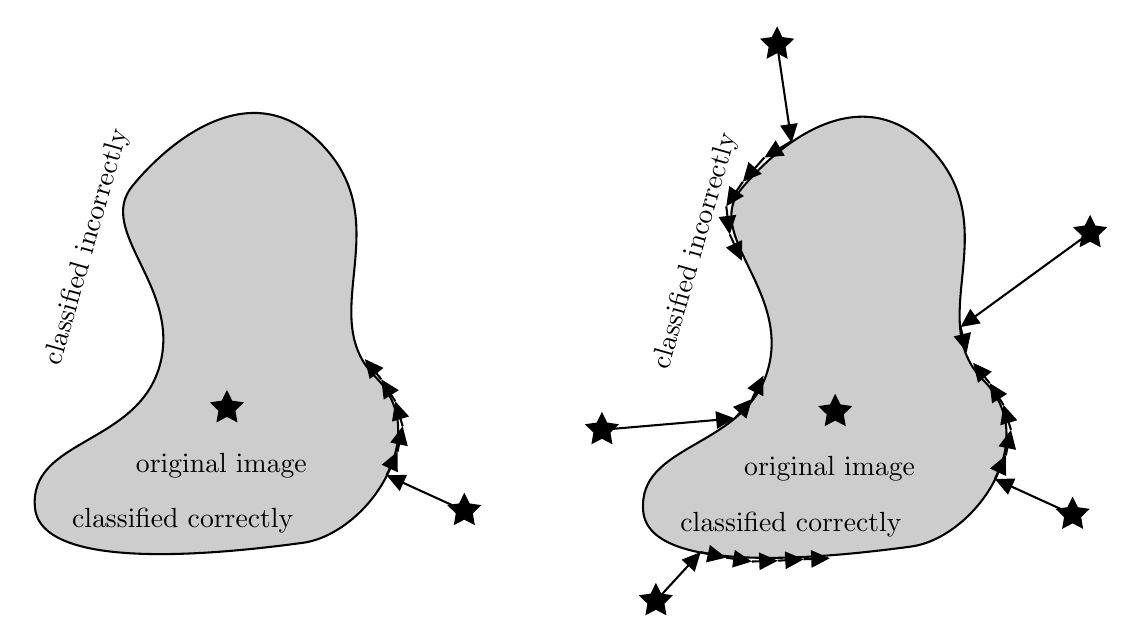
\begin{tikzpicture}[x=0.75pt,y=0.75pt,yscale=-1,xscale=1]
%uncomment if require: \path (0,300); %set diagram left start at 0, and has height of 300

%Shape: Polygon Curved [id:ds39418321723754923] 
\draw  [fill={rgb, 255:red, 155; green, 155; blue, 155 }  ,fill opacity=0.5 ] (365.12,90.5) .. controls (383.12,68.5) and (424.12,34.5) .. (458.12,72.5) .. controls (492.12,110.5) and (453.12,153.5) .. (482.12,182.5) .. controls (511.12,211.5) and (477.12,258.5) .. (447.12,262.5) .. controls (417.12,266.5) and (321.12,278.5) .. (318.12,245.5) .. controls (315.12,212.5) and (367.12,215.5) .. (378.12,177.5) .. controls (389.12,139.5) and (347.12,112.5) .. (365.12,90.5) -- cycle ;
%Shape: Star [id:dp17995230177708343] 
\draw  [fill={rgb, 255:red, 0; green, 0; blue, 0 }  ,fill opacity=1 ] (410.62,190) -- (412.83,194.47) -- (417.76,195.18) -- (414.19,198.66) -- (415.03,203.57) -- (410.62,201.25) -- (406.22,203.57) -- (407.06,198.66) -- (403.49,195.18) -- (408.42,194.47) -- cycle ;
%Shape: Star [id:dp263511542953333] 
\draw  [fill={rgb, 255:red, 0; green, 0; blue, 0 }  ,fill opacity=1 ] (382.62,13) -- (384.83,17.47) -- (389.76,18.18) -- (386.19,21.66) -- (387.03,26.57) -- (382.62,24.25) -- (378.22,26.57) -- (379.06,21.66) -- (375.49,18.18) -- (380.42,17.47) -- cycle ;
%Straight Lines [id:da12241666866362477] 
\draw    (382.62,20.5) -- (389.19,64.95) ;
\draw [shift={(389.62,67.92)}, rotate = 261.6] [fill={rgb, 255:red, 0; green, 0; blue, 0 }  ][line width=0.08]  [draw opacity=0] (8.93,-4.29) -- (0,0) -- (8.93,4.29) -- cycle    ;
%Straight Lines [id:da7985170559413728] 
\draw    (389.79,67.08) -- (379.03,73.54) ;
\draw [shift={(376.46,75.08)}, rotate = 329.04] [fill={rgb, 255:red, 0; green, 0; blue, 0 }  ][line width=0.08]  [draw opacity=0] (8.93,-4.29) -- (0,0) -- (8.93,4.29) -- cycle    ;
%Straight Lines [id:da5286207592270582] 
\draw    (376.46,75.08) -- (368.11,84.5) ;
\draw [shift={(366.12,86.75)}, rotate = 311.53] [fill={rgb, 255:red, 0; green, 0; blue, 0 }  ][line width=0.08]  [draw opacity=0] (8.93,-4.29) -- (0,0) -- (8.93,4.29) -- cycle    ;
%Straight Lines [id:da4098354744836743] 
\draw    (366.12,86.75) -- (359.8,96.1) ;
\draw [shift={(358.12,98.58)}, rotate = 304.06] [fill={rgb, 255:red, 0; green, 0; blue, 0 }  ][line width=0.08]  [draw opacity=0] (8.93,-4.29) -- (0,0) -- (8.93,4.29) -- cycle    ;
%Straight Lines [id:da7402027038712158] 
\draw    (358.12,98.58) -- (359.42,109.11) ;
\draw [shift={(359.79,112.08)}, rotate = 262.96] [fill={rgb, 255:red, 0; green, 0; blue, 0 }  ][line width=0.08]  [draw opacity=0] (8.93,-4.29) -- (0,0) -- (8.93,4.29) -- cycle    ;
%Straight Lines [id:da22742294505428506] 
\draw    (359.79,112.08) -- (364.37,122.03) ;
\draw [shift={(365.62,124.75)}, rotate = 245.27] [fill={rgb, 255:red, 0; green, 0; blue, 0 }  ][line width=0.08]  [draw opacity=0] (8.93,-4.29) -- (0,0) -- (8.93,4.29) -- cycle    ;
%Shape: Boxed Line [id:dp17555971988752717] 
\draw    (362.2,200.74) -- (368.55,193.64) ;
\draw [shift={(370.55,191.4)}, rotate = 131.8] [fill={rgb, 255:red, 0; green, 0; blue, 0 }  ][line width=0.08]  [draw opacity=0] (8.93,-4.29) -- (0,0) -- (8.93,4.29) -- cycle    ;
%Shape: Star [id:dp5469311004467188] 
\draw  [fill={rgb, 255:red, 0; green, 0; blue, 0 }  ,fill opacity=1 ] (533.42,103.8) -- (535.63,108.27) -- (540.56,108.98) -- (536.99,112.46) -- (537.83,117.37) -- (533.42,115.05) -- (529.02,117.37) -- (529.86,112.46) -- (526.29,108.98) -- (531.22,108.27) -- cycle ;
%Shape: Star [id:dp8199494411723183] 
\draw  [fill={rgb, 255:red, 0; green, 0; blue, 0 }  ,fill opacity=1 ] (525,239.51) -- (527.2,243.97) -- (532.13,244.69) -- (528.57,248.17) -- (529.41,253.07) -- (525,250.76) -- (520.59,253.07) -- (521.43,248.17) -- (517.87,244.69) -- (522.8,243.97) -- cycle ;
%Shape: Star [id:dp3621439940158031] 
\draw  [fill={rgb, 255:red, 0; green, 0; blue, 0 }  ,fill opacity=1 ] (324.22,281.14) -- (326.43,285.61) -- (331.36,286.32) -- (327.79,289.8) -- (328.63,294.71) -- (324.22,292.39) -- (319.82,294.71) -- (320.66,289.8) -- (317.09,286.32) -- (322.02,285.61) -- cycle ;
%Shape: Star [id:dp886425904787334] 
\draw  [fill={rgb, 255:red, 0; green, 0; blue, 0 }  ,fill opacity=1 ] (298.22,198.74) -- (300.43,203.21) -- (305.36,203.92) -- (301.79,207.4) -- (302.63,212.31) -- (298.22,209.99) -- (293.82,212.31) -- (294.66,207.4) -- (291.09,203.92) -- (296.02,203.21) -- cycle ;
%Straight Lines [id:da29737150039250193] 
\draw    (533.42,111.3) -- (473.43,154.98) ;
\draw [shift={(471,156.74)}, rotate = 323.95] [fill={rgb, 255:red, 0; green, 0; blue, 0 }  ][line width=0.08]  [draw opacity=0] (8.93,-4.29) -- (0,0) -- (8.93,4.29) -- cycle    ;
%Straight Lines [id:da564242749820822] 
\draw    (298.22,206.24) -- (359.21,201) ;
\draw [shift={(362.2,200.74)}, rotate = 175.09] [fill={rgb, 255:red, 0; green, 0; blue, 0 }  ][line width=0.08]  [draw opacity=0] (8.93,-4.29) -- (0,0) -- (8.93,4.29) -- cycle    ;
%Straight Lines [id:da8824188996602935] 
\draw    (525,247.01) -- (490.26,231.18) ;
\draw [shift={(487.53,229.94)}, rotate = 24.49] [fill={rgb, 255:red, 0; green, 0; blue, 0 }  ][line width=0.08]  [draw opacity=0] (8.93,-4.29) -- (0,0) -- (8.93,4.29) -- cycle    ;
%Straight Lines [id:da172043009485096] 
\draw    (324.22,288.64) -- (343.77,267.35) ;
\draw [shift={(345.8,265.14)}, rotate = 132.55] [fill={rgb, 255:red, 0; green, 0; blue, 0 }  ][line width=0.08]  [draw opacity=0] (8.93,-4.29) -- (0,0) -- (8.93,4.29) -- cycle    ;
%Shape: Boxed Line [id:dp5913488094519332] 
\draw    (370.55,191.4) -- (374.75,182.84) ;
\draw [shift={(376.07,180.15)}, rotate = 116.11] [fill={rgb, 255:red, 0; green, 0; blue, 0 }  ][line width=0.08]  [draw opacity=0] (8.93,-4.29) -- (0,0) -- (8.93,4.29) -- cycle    ;
%Shape: Boxed Line [id:dp8616221435272089] 
\draw    (487.53,229.94) -- (491.55,221.3) ;
\draw [shift={(492.81,218.58)}, rotate = 114.93] [fill={rgb, 255:red, 0; green, 0; blue, 0 }  ][line width=0.08]  [draw opacity=0] (8.93,-4.29) -- (0,0) -- (8.93,4.29) -- cycle    ;
%Shape: Boxed Line [id:dp5796326247856174] 
\draw    (492.81,218.58) -- (494.7,209.24) ;
\draw [shift={(495.29,206.29)}, rotate = 101.39] [fill={rgb, 255:red, 0; green, 0; blue, 0 }  ][line width=0.08]  [draw opacity=0] (8.93,-4.29) -- (0,0) -- (8.93,4.29) -- cycle    ;
%Shape: Boxed Line [id:dp044334919963415986] 
\draw    (495.29,206.29) -- (492.57,197.16) ;
\draw [shift={(491.71,194.29)}, rotate = 73.42] [fill={rgb, 255:red, 0; green, 0; blue, 0 }  ][line width=0.08]  [draw opacity=0] (8.93,-4.29) -- (0,0) -- (8.93,4.29) -- cycle    ;
%Shape: Boxed Line [id:dp4387546700476397] 
\draw    (491.71,194.29) -- (486.61,186.24) ;
\draw [shift={(485,183.71)}, rotate = 57.58] [fill={rgb, 255:red, 0; green, 0; blue, 0 }  ][line width=0.08]  [draw opacity=0] (8.93,-4.29) -- (0,0) -- (8.93,4.29) -- cycle    ;
%Shape: Boxed Line [id:dp8947094222533136] 
\draw    (485,183.71) -- (478.98,176.32) ;
\draw [shift={(477.09,173.99)}, rotate = 50.85] [fill={rgb, 255:red, 0; green, 0; blue, 0 }  ][line width=0.08]  [draw opacity=0] (8.93,-4.29) -- (0,0) -- (8.93,4.29) -- cycle    ;
%Shape: Boxed Line [id:dp8126738394252795] 
\draw    (471,156.74) -- (473.27,166) ;
\draw [shift={(473.99,168.91)}, rotate = 256.19] [fill={rgb, 255:red, 0; green, 0; blue, 0 }  ][line width=0.08]  [draw opacity=0] (8.93,-4.29) -- (0,0) -- (8.93,4.29) -- cycle    ;
%Shape: Boxed Line [id:dp14754319972001273] 
\draw    (345.8,265.14) -- (355.11,267.18) ;
\draw [shift={(358.04,267.82)}, rotate = 192.33] [fill={rgb, 255:red, 0; green, 0; blue, 0 }  ][line width=0.08]  [draw opacity=0] (8.93,-4.29) -- (0,0) -- (8.93,4.29) -- cycle    ;
%Shape: Boxed Line [id:dp8374639915608668] 
\draw    (358.04,267.82) -- (367.46,269.26) ;
\draw [shift={(370.43,269.71)}, rotate = 188.71] [fill={rgb, 255:red, 0; green, 0; blue, 0 }  ][line width=0.08]  [draw opacity=0] (8.93,-4.29) -- (0,0) -- (8.93,4.29) -- cycle    ;
%Shape: Boxed Line [id:dp496623104677657] 
\draw    (370.43,269.71) -- (379.95,269.39) ;
\draw [shift={(382.95,269.29)}, rotate = 178.04] [fill={rgb, 255:red, 0; green, 0; blue, 0 }  ][line width=0.08]  [draw opacity=0] (8.93,-4.29) -- (0,0) -- (8.93,4.29) -- cycle    ;
%Shape: Boxed Line [id:dp34473561543285314] 
\draw    (382.95,269.29) -- (392.47,268.77) ;
\draw [shift={(395.46,268.61)}, rotate = 176.92] [fill={rgb, 255:red, 0; green, 0; blue, 0 }  ][line width=0.08]  [draw opacity=0] (8.93,-4.29) -- (0,0) -- (8.93,4.29) -- cycle    ;
%Shape: Boxed Line [id:dp22829712791209555] 
\draw    (395.46,268.61) -- (404.98,268.23) ;
\draw [shift={(407.98,268.11)}, rotate = 177.71] [fill={rgb, 255:red, 0; green, 0; blue, 0 }  ][line width=0.08]  [draw opacity=0] (8.93,-4.29) -- (0,0) -- (8.93,4.29) -- cycle    ;

%Shape: Polygon Curved [id:ds013419098702227128] 
\draw  [fill={rgb, 255:red, 155; green, 155; blue, 155 }  ,fill opacity=0.5 ] (72.05,88.7) .. controls (90.05,66.7) and (131.05,32.7) .. (165.05,70.7) .. controls (199.05,108.7) and (160.05,151.7) .. (189.05,180.7) .. controls (218.05,209.7) and (184.05,256.7) .. (154.05,260.7) .. controls (124.05,264.7) and (28.05,276.7) .. (25.05,243.7) .. controls (22.05,210.7) and (74.05,213.7) .. (85.05,175.7) .. controls (96.05,137.7) and (54.05,110.7) .. (72.05,88.7) -- cycle ;
%Shape: Star [id:dp9534459695500062] 
\draw  [fill={rgb, 255:red, 0; green, 0; blue, 0 }  ,fill opacity=1 ] (117.55,188.2) -- (119.76,192.67) -- (124.68,193.38) -- (121.12,196.86) -- (121.96,201.77) -- (117.55,199.45) -- (113.14,201.77) -- (113.99,196.86) -- (110.42,193.38) -- (115.35,192.67) -- cycle ;
%Shape: Star [id:dp3150974101447812] 
\draw  [fill={rgb, 255:red, 0; green, 0; blue, 0 }  ,fill opacity=1 ] (231.93,237.71) -- (234.13,242.17) -- (239.06,242.89) -- (235.49,246.37) -- (236.34,251.28) -- (231.93,248.96) -- (227.52,251.28) -- (228.36,246.37) -- (224.79,242.89) -- (229.72,242.17) -- cycle ;
%Straight Lines [id:da8721626382201679] 
\draw    (231.93,245.21) -- (197.19,229.38) ;
\draw [shift={(194.46,228.14)}, rotate = 24.49] [fill={rgb, 255:red, 0; green, 0; blue, 0 }  ][line width=0.08]  [draw opacity=0] (8.93,-4.29) -- (0,0) -- (8.93,4.29) -- cycle    ;
%Shape: Boxed Line [id:dp35233924811215767] 
\draw    (194.46,228.14) -- (198.48,219.5) ;
\draw [shift={(199.74,216.78)}, rotate = 114.93] [fill={rgb, 255:red, 0; green, 0; blue, 0 }  ][line width=0.08]  [draw opacity=0] (8.93,-4.29) -- (0,0) -- (8.93,4.29) -- cycle    ;
%Shape: Boxed Line [id:dp47377705399021885] 
\draw    (199.74,216.78) -- (201.62,207.44) ;
\draw [shift={(202.22,204.5)}, rotate = 101.39] [fill={rgb, 255:red, 0; green, 0; blue, 0 }  ][line width=0.08]  [draw opacity=0] (8.93,-4.29) -- (0,0) -- (8.93,4.29) -- cycle    ;
%Shape: Boxed Line [id:dp01327277725498055] 
\draw    (202.22,204.5) -- (199.5,195.36) ;
\draw [shift={(198.64,192.49)}, rotate = 73.42] [fill={rgb, 255:red, 0; green, 0; blue, 0 }  ][line width=0.08]  [draw opacity=0] (8.93,-4.29) -- (0,0) -- (8.93,4.29) -- cycle    ;
%Shape: Boxed Line [id:dp6860848467619505] 
\draw    (198.64,192.49) -- (193.53,184.44) ;
\draw [shift={(191.92,181.91)}, rotate = 57.58] [fill={rgb, 255:red, 0; green, 0; blue, 0 }  ][line width=0.08]  [draw opacity=0] (8.93,-4.29) -- (0,0) -- (8.93,4.29) -- cycle    ;
%Shape: Boxed Line [id:dp2849658598230065] 
\draw    (191.92,181.91) -- (185.91,174.52) ;
\draw [shift={(184.01,172.19)}, rotate = 50.85] [fill={rgb, 255:red, 0; green, 0; blue, 0 }  ][line width=0.08]  [draw opacity=0] (8.93,-4.29) -- (0,0) -- (8.93,4.29) -- cycle    ;


% Text Node
\draw (107.14,250.13) node   [align=left] {\begin{minipage}[lt]{96.27pt}\setlength\topsep{0pt}
classified correctly
\end{minipage}};
% Text Node
\draw (51.61,113.14) node  [rotate=-286.01] [align=left] {\begin{minipage}[lt]{96.27pt}\setlength\topsep{0pt}
classified incorrectly
\end{minipage}};
% Text Node
\draw (119.05,223.33) node   [align=left] {\begin{minipage}[lt]{68pt}\setlength\topsep{0pt}
original image
\end{minipage}};
% Text Node
\draw (400.21,251.93) node   [align=left] {\begin{minipage}[lt]{96.27pt}\setlength\topsep{0pt}
classified correctly
\end{minipage}};
% Text Node
\draw (344.71,114.94) node  [rotate=-286.01] [align=left] {\begin{minipage}[lt]{96.27pt}\setlength\topsep{0pt}
classified incorrectly
\end{minipage}};
% Text Node
\draw (412.12,225.13) node   [align=left] {\begin{minipage}[lt]{68pt}\setlength\topsep{0pt}
original image
\end{minipage}};


\end{tikzpicture}	
\caption[Intuition of multiple starting points]{The vanilla version of \gls{bba} might get stuck in a local optimum depending on the starting point (left plot). By starting from multiple positions, the probability that \gls{bba} gets stuck in a local optimum is reduced (right plot). The multiple starting points are particles in a \gls{pso} swarm.}
\label{fig:applying_pso_to_bba}
\end{figure}

\begin{figure}
\centering
\begin{tikzpicture}
\begin{axis}[width=12cm, height=5cm, xmin=0,xmax=25000, xlabel=Calls, ylabel=Detections, tick label style={/pgf/number format/fixed}, scaled ticks=false, enlarge x limits=0.01, xtick={0,5000,10000,15000,20000,25000},legend pos=north west,	legend style={draw=none},]
\addplot table[col sep=comma,x index=1,y expr=\thisrowno{0} + 1,mark=none] {Data/detections_bba.csv};
\addlegendentry{\gls{bba}};
\addplot table[col sep=comma,x index=1,y expr=\thisrowno{0} + 1,mark=none] {Data/detections_pso_bba.csv};
\addlegendentry{\gls{pso}-\gls{bba}};

\end{axis}
\end{tikzpicture}
\caption[Detections of the different attacks]{The cumulative number of detections for different attack algorithms for one specific experiment. The number of detections of the \gls{bba} algorithm steadily increases with the number of calls. The number of detections of the \gls{pso}-\gls{bba} algorithm increases more slowly in the beginning due to the dispersed nature of the attack. The increase is more sharp near the end of the attack.}
\label{fig:detections_bba_vs_pso_bba}
\end{figure}

\begin{table}
	\centering
	\caption[PSO-BBA results]{Results for the \gls{pso}-\gls{bba} approach on MNIST and CIFAR-10 dataset.}
	\label{tbl:pso_bba}
	\begin{tabular}{lrrrr}\toprule
			& \multicolumn{2}{c}{MNIST} &\multicolumn{2}{c}{CIFAR} \\ \cmidrule(r){2-3} \cmidrule(r){4-5}
	Attack				&Distance	&Detections	&Distance	&Detections \\ \midrule
	Baseline \gls{bba}	&3.027		&339		&1.359			&475 \\
	\gls{pso}-\gls{bba} (5 particles)	&2.884			&79			&1.133				&301 \\ 
	\gls{pso}-\gls{bba} (10 particles)	&2.788			&107			&1.782				&243 \\
	\bottomrule
	
	\end{tabular}
\end{table}

\section{Towards distribution of the attack}


\section{Throwing the defense off the scent}

\section{Optimizing the attack}
